\documentclass[11pt,a4paper]{article}
\usepackage[a4paper,margin=0.72in]{geometry}
\usepackage[T1]{fontenc}
\usepackage[utf8]{inputenc}
\usepackage{lmodern}
\usepackage{amsmath,amssymb,mathtools}
\usepackage{array,booktabs,longtable,multicol}
\usepackage{enumitem}
\usepackage{xcolor}
\usepackage{tikz}
\usetikzlibrary{arrows.meta,calc,positioning,patterns}
\usepackage{fancyhdr}
\usepackage{hyperref}
\usepackage[most]{tcolorbox}
\hypersetup{colorlinks=true,linkcolor=blue!50!black,urlcolor=blue!50!black}

\definecolor{headblue}{HTML}{123B5D}
\definecolor{softblue}{HTML}{EAF4FF}
\definecolor{softgreen}{HTML}{EDF9F1}
\definecolor{softyellow}{HTML}{FFF8E1}
\definecolor{linegray}{HTML}{666666}

\pagestyle{fancy}
\fancyhf{}
\lhead{\textbf{BCS-012: Basic Mathematics}}
\rhead{\textbf{Solved Paper: December 2023}}
\cfoot{\thepage}
\renewcommand{\headrulewidth}{0.4pt}
\setlength{\headheight}{14pt}

\setlength{\parindent}{0pt}
\setlength{\parskip}{5pt}
\setlist[enumerate]{leftmargin=*,itemsep=4pt,topsep=3pt}
\newcommand{\question}[1]{\vspace{4pt}\begin{tcolorbox}[colback=softblue,colframe=headblue,boxrule=0.6pt,arc=2pt,left=5pt,right=5pt,top=4pt,bottom=4pt]\textbf{#1}\end{tcolorbox}}
\newcommand{\answer}{\textbf{Solution.}~}
\newcommand{\finalans}[1]{\[\boxed{#1}\]}

\begin{document}

\begin{center}
{\Large\bfseries IGNOU BCS-012: Basic Mathematics}\\[2mm]
{\large\bfseries Term-End Examination, December 2023 - Full Solved Paper}\\[1mm]
Time: 3 Hours \quad Maximum Marks: 100\par
\end{center}

\begin{tcolorbox}[colback=softyellow,colframe=orange!70!black,title=How to use this solved paper]
Question 1 is compulsory. In the actual examination, any three questions are attempted from Questions 2--5. Here, all questions have been solved for complete practice. A compact theory and formula sheet is given at the end.
\end{tcolorbox}

\section*{Question 1}

\question{1(a). Show that
\[
\begin{vmatrix}
b-c&c-a&a-b\\
c-a&a-b&b-c\\
a-b&b-c&c-a
\end{vmatrix}=0.
\]}
\answer
Add the elements of the first row:
\[
(b-c)+(c-a)+(a-b)=0.
\]
Similarly, the sum of every row is zero. Therefore, if the three columns are added, we get a zero column:
\[
C_1+C_2+C_3=0.
\]
Thus the columns are linearly dependent. Hence the determinant is zero.
\finalans{0}

\question{1(b). If
\[
A=\begin{bmatrix}2&3\\-1&2\end{bmatrix},\qquad f(x)=x^2-4x+7,
\]
show that $f(A)=O_{2\times2}$. Use this result to find $A^5$.}
\answer
First,
\[
A^2=\begin{bmatrix}2&3\\-1&2\end{bmatrix}
\begin{bmatrix}2&3\\-1&2\end{bmatrix}
=\begin{bmatrix}1&12\\-4&1\end{bmatrix}.
\]
Hence
\[
f(A)=A^2-4A+7I
=\begin{bmatrix}1&12\\-4&1\end{bmatrix}
-\begin{bmatrix}8&12\\-4&8\end{bmatrix}
+\begin{bmatrix}7&0\\0&7\end{bmatrix}
=\begin{bmatrix}0&0\\0&0\end{bmatrix}.
\]
Thus
\[
A^2-4A+7I=0\quad\Rightarrow\quad A^2=4A-7I.
\]
Now,
\[
A^3=A(4A-7I)=4A^2-7A=4(4A-7I)-7A=9A-28I,
\]
\[
A^4=A(9A-28I)=9A^2-28A=9(4A-7I)-28A=8A-63I,
\]
\[
A^5=A(8A-63I)=8A^2-63A=8(4A-7I)-63A=-31A-56I.
\]
Therefore,
\[
A^5=-31\begin{bmatrix}2&3\\-1&2\end{bmatrix}-56\begin{bmatrix}1&0\\0&1\end{bmatrix}
=\begin{bmatrix}-118&-93\\31&-118\end{bmatrix}.
\]
\finalans{A^5=\begin{bmatrix}-118&-93\\31&-118\end{bmatrix}}

\question{1(c). Show that $7$ divides $2^{3n}-1$ for every $n\in\mathbb{N}$.}
\answer
Since $2^3=8$, we have
\[
2^{3n}-1=8^n-1.
\]
Now $8\equiv1\pmod 7$. Therefore,
\[
8^n\equiv1^n\equiv1\pmod 7.
\]
Thus
\[
8^n-1\equiv0\pmod 7.
\]
Hence $7$ divides $2^{3n}-1$ for every natural number $n$.
\finalans{7\mid(2^{3n}-1)}

\question{1(d). If $1,\omega,\omega^2$ are cube roots of unity, show that
\[
(1+\omega)(1+\omega^2)(1+\omega^3)(1+\omega^4)(1+\omega^6)(1+\omega^8)=4.
\]}
\answer
For cube roots of unity,
\[
\omega^3=1,\qquad 1+\omega+\omega^2=0.
\]
Reduce powers modulo $3$:
\[
\omega^3=1,
\quad \omega^4=\omega,
\quad \omega^6=1,
\quad \omega^8=\omega^2.
\]
Therefore,
\[
(1+\omega)(1+\omega^2)(1+\omega^3)(1+\omega^4)(1+\omega^6)(1+\omega^8)
\]
\[
=(1+\omega)(1+\omega^2)(2)(1+\omega)(2)(1+\omega^2).
\]
Also,
\[
(1+\omega)(1+\omega^2)=1+\omega+\omega^2+\omega^3
=1+(-1)+1=1.
\]
Hence the product is
\[
4\{(1+\omega)(1+\omega^2)\}^2=4.
\]
\finalans{4}

\question{1(e). If $y=ae^{mx}+be^{-mx}+4$, show that
\[
\frac{d^2y}{dx^2}=m^2(y-4).
\]}
\answer
Given
\[
y=ae^{mx}+be^{-mx}+4.
\]
Then
\[
\frac{dy}{dx}=am e^{mx}-bm e^{-mx},
\]
\[
\frac{d^2y}{dx^2}=am^2e^{mx}+bm^2e^{-mx}
=m^2(ae^{mx}+be^{-mx}).
\]
But
\[
y-4=ae^{mx}+be^{-mx}.
\]
Therefore,
\[
\frac{d^2y}{dx^2}=m^2(y-4).
\]
\finalans{\dfrac{d^2y}{dx^2}=m^2(y-4)}

\question{1(f). If $\alpha,\beta$ are roots of
\[
x^2-2kx+k^2-1=0
\]
and $\alpha^2+\beta^2=10$, find $k$.}
\answer
For the quadratic equation,
\[
\alpha+\beta=2k,
\qquad \alpha\beta=k^2-1.
\]
Now
\[
\alpha^2+\beta^2=(\alpha+\beta)^2-2\alpha\beta.
\]
Thus
\[
10=(2k)^2-2(k^2-1)=4k^2-2k^2+2=2k^2+2.
\]
So
\[
2k^2=8\quad\Rightarrow\quad k^2=4.
\]
\finalans{k=\pm2}

\question{1(g). Find the value of $\lambda$ for which the vectors
\[
\vec a=2\hat i-4\hat j+3\hat k,\quad
\vec b=\lambda\hat i-2\hat j+\hat k,
\quad \vec c=2\hat i+3\hat j+3\hat k
\]
are coplanar.}
\answer
Three vectors are coplanar if their scalar triple product is zero:
\[
[\vec a\ \vec b\ \vec c]=0.
\]
Thus
\[
\begin{vmatrix}
2&-4&3\\
\lambda&-2&1\\
2&3&3
\end{vmatrix}=0.
\]
Expanding,
\[
2\begin{vmatrix}-2&1\\3&3\end{vmatrix}
+4\begin{vmatrix}\lambda&1\\2&3\end{vmatrix}
+3\begin{vmatrix}\lambda&-2\\2&3\end{vmatrix}=0.
\]
\[
2(-9)+4(3\lambda-2)+3(3\lambda+4)=0.
\]
\[
-18+12\lambda-8+9\lambda+12=0
\quad\Rightarrow\quad 21\lambda-14=0.
\]
\finalans{\lambda=\frac{2}{3}}

\question{1(h). Find the angle between the pair of lines
\[
\frac{x-5}{2}=\frac{y-3}{3}=\frac{z-1}{-3}
\]
and
\[
\frac{x}{3}=\frac{y-1}{2}=\frac{z+5}{-3}.
\]}
\answer
The direction ratios of the two lines are
\[
\vec d_1=(2,3,-3),\qquad \vec d_2=(3,2,-3).
\]
The angle $\theta$ between the lines is the angle between their direction vectors:
\[
\cos\theta=\frac{|\vec d_1\cdot \vec d_2|}{|\vec d_1||\vec d_2|}.
\]
Now
\[
\vec d_1\cdot \vec d_2=2\cdot3+3\cdot2+(-3)(-3)=21,
\]
\[
|\vec d_1|=\sqrt{4+9+9}=\sqrt{22},
\quad |\vec d_2|=\sqrt{9+4+9}=\sqrt{22}.
\]
Therefore,
\[
\cos\theta=\frac{21}{22}.
\]
\finalans{\theta=\cos^{-1}\left(\frac{21}{22}\right)}

\section*{Question 2}

\question{2(a). Solve the following set of linear equations by using matrix inverse:
\[
3x+4y+7z=-2,
\quad 2x-y+3z=6,
\quad 2x+2y-3z=0.
\]}
\answer
Write the system as $AX=B$, where
\[
A=\begin{bmatrix}3&4&7\\2&-1&3\\2&2&-3\end{bmatrix},
\quad
X=\begin{bmatrix}x\\y\\z\end{bmatrix},
\quad
B=\begin{bmatrix}-2\\6\\0\end{bmatrix}.
\]
The inverse method gives
\[
X=A^{-1}B.
\]
Solving, we obtain
\[
\begin{bmatrix}x\\y\\z\end{bmatrix}
=
\begin{bmatrix}2\\-2\\0\end{bmatrix}.
\]
Verification:
\[
3(2)+4(-2)+7(0)=-2,
\]
\[
2(2)-(-2)+3(0)=6,
\]
\[
2(2)+2(-2)-3(0)=0.
\]
\finalans{x=2,\quad y=-2,\quad z=0}

\question{2(b). Use the principle of mathematical induction to prove that
\[
1^3+2^3+\cdots+n^3=\frac{1}{4}n^2(n+1)^2
\]
for every natural number $n$.}
\answer
Let
\[
P(n):1^3+2^3+\cdots+n^3=\frac{n^2(n+1)^2}{4}.
\]
For $n=1$,
\[
1^3=1=\frac{1^2(1+1)^2}{4}.
\]
So $P(1)$ is true.

Assume $P(k)$ is true:
\[
1^3+2^3+\cdots+k^3=\frac{k^2(k+1)^2}{4}.
\]
Then
\[
1^3+2^3+\cdots+k^3+(k+1)^3
=\frac{k^2(k+1)^2}{4}+(k+1)^3.
\]
\[
=(k+1)^2\left(\frac{k^2}{4}+k+1\right)
=(k+1)^2\left(\frac{k^2+4k+4}{4}\right).
\]
\[
=\frac{(k+1)^2(k+2)^2}{4}.
\]
This is the required formula for $n=k+1$. Therefore, by induction, the result holds for every $n\in\mathbb N$.
\finalans{1^3+2^3+\cdots+n^3=\left(\frac{n(n+1)}{2}\right)^2}

\question{2(c). Find how many terms of the GP
\[
\sqrt3,\ 3,\ 3\sqrt3,\ldots
\]
add up to $120+40\sqrt3$.}
\answer
Here
\[
a=\sqrt3,
\qquad r=\frac{3}{\sqrt3}=\sqrt3.
\]
The sum of $n$ terms is
\[
S_n=\frac{a(r^n-1)}{r-1}
=\frac{\sqrt3\{(\sqrt3)^n-1\}}{\sqrt3-1}.
\]
Check the sum of the first eight terms:
\[
\sqrt3+3+3\sqrt3+9+9\sqrt3+27+27\sqrt3+81.
\]
Separate rational and irrational parts:
\[
(3+9+27+81)+(1+3+9+27)\sqrt3=120+40\sqrt3.
\]
Hence the required number of terms is eight.
\finalans{n=8}

\question{2(d). Write De Moivre's theorem and use it to find $(i+\sqrt3)^3$.}
\answer
De Moivre's theorem states that if $n$ is an integer, then
\[
(\cos\theta+i\sin\theta)^n=\cos n\theta+i\sin n\theta.
\]
Now
\[
i+\sqrt3=\sqrt3+i.
\]
Its modulus is
\[
r=\sqrt{(\sqrt3)^2+1^2}=2.
\]
Also
\[
\cos\theta=\frac{\sqrt3}{2},\qquad \sin\theta=\frac12,
\]
so $\theta=\pi/6$. Therefore,
\[
\sqrt3+i=2\left(\cos\frac{\pi}{6}+i\sin\frac{\pi}{6}\right).
\]
Thus
\[
(i+\sqrt3)^3=2^3\left(\cos\frac{3\pi}{6}+i\sin\frac{3\pi}{6}\right)
=8\left(\cos\frac{\pi}{2}+i\sin\frac{\pi}{2}\right)=8i.
\]
\finalans{(i+\sqrt3)^3=8i}

\section*{Question 3}

\question{3(a). If
\[
A=\begin{bmatrix}-1&2&3\\4&5&7\\5&3&4\end{bmatrix},
\]
show that $A(\operatorname{adj}A)=0$.}
\answer
We know that
\[
A(\operatorname{adj}A)=|A|I.
\]
So it is enough to show that $|A|=0$.
\[
|A|=\begin{vmatrix}-1&2&3\\4&5&7\\5&3&4\end{vmatrix}.
\]
Expanding along the first row,
\[
|A|=-1\begin{vmatrix}5&7\\3&4\end{vmatrix}
-2\begin{vmatrix}4&7\\5&4\end{vmatrix}
+3\begin{vmatrix}4&5\\5&3\end{vmatrix}.
\]
\[
=-1(20-21)-2(16-35)+3(12-25)
=1+38-39=0.
\]
Therefore,
\[
A(\operatorname{adj}A)=|A|I=0I=0.
\]
\finalans{A(\operatorname{adj}A)=0}

\question{3(b). Solve the inequality
\[
\left|\frac{x-4}{2}\right|\leq\frac{5}{12}
\]
and graph the solution set.}
\answer
\[
\left|\frac{x-4}{2}\right|\leq\frac{5}{12}
\quad\Rightarrow\quad
|x-4|\leq\frac{5}{6}.
\]
Thus
\[
-\frac56\leq x-4\leq\frac56.
\]
Adding $4$ throughout,
\[
4-\frac56\leq x\leq4+\frac56.
\]
Therefore,
\[
\frac{19}{6}\leq x\leq\frac{29}{6}.
\]

\begin{center}
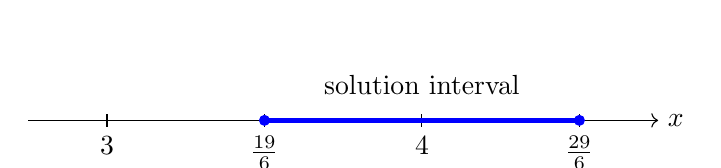
\begin{tikzpicture}[scale=1]
\draw[->] (0,0) -- (8,0) node[right] {$x$};
\foreach \x/\lab in {1/3,3/\frac{19}{6},5/4,7/\frac{29}{6}}
{\draw (\x,0.08)--(\x,-0.08) node[below] {$\lab$};}
\draw[line width=2pt,blue] (3,0) -- (7,0);
\fill[blue] (3,0) circle (2pt);
\fill[blue] (7,0) circle (2pt);
\node[above] at (5,0.2) {solution interval};
\end{tikzpicture}
\end{center}

\finalans{x\in\left[\frac{19}{6},\frac{29}{6}\right]}

\question{3(c). Solve the equation
\[
8x^3-14x^2+7x-1=0,
\]
given that the roots are in GP.}
\answer
We factor the polynomial:
\[
8x^3-14x^2+7x-1
=(x-1)(2x-1)(4x-1).
\]
Therefore,
\[
(x-1)(2x-1)(4x-1)=0.
\]
So
\[
x=1,\quad x=\frac12,\quad x=\frac14.
\]
These roots are in GP because
\[
\frac{1/2}{1/4}=2,
\qquad \frac{1}{1/2}=2.
\]
\finalans{x=\frac14,\ \frac12,\ 1}

\question{3(d). Verify that
\[
f(x)=1+x^2\ln\left(\frac1x\right)
\]
has a local maxima at $x=\frac1{\sqrt e}$, $x>0$.}
\answer
Since
\[
\ln\left(\frac1x\right)=-\ln x,
\]
we write
\[
f(x)=1-x^2\ln x.
\]
Then
\[
f'(x)=-(2x\ln x+x)=-x(2\ln x+1).
\]
For a stationary point,
\[
f'(x)=0.
\]
Since $x>0$,
\[
2\ln x+1=0
\quad\Rightarrow\quad
\ln x=-\frac12
\quad\Rightarrow\quad
x=e^{-1/2}=\frac1{\sqrt e}.
\]
Now
\[
f''(x)=-(2\ln x+3).
\]
At $x=1/\sqrt e$,
\[
\ln x=-\frac12,
\quad
f''(x)=-\{-1+3\}=-2<0.
\]
Hence $f(x)$ has a local maximum at $x=1/\sqrt e$.
The maximum value is
\[
f\left(\frac1{\sqrt e}\right)=1+\frac1e\cdot\frac12=1+\frac1{2e}.
\]
\finalans{\text{Local maximum at }x=\frac1{\sqrt e},\quad f_{\max}=1+\frac1{2e}}

\section*{Question 4}

\question{4(a). Evaluate
\[
\lim_{x\to0}\frac{\sqrt{1+2x}-\sqrt{1-2x}}{x}.
\]}
\answer
Rationalise the numerator:
\[
\frac{\sqrt{1+2x}-\sqrt{1-2x}}{x}
\cdot
\frac{\sqrt{1+2x}+\sqrt{1-2x}}{\sqrt{1+2x}+\sqrt{1-2x}}.
\]
This gives
\[
\frac{(1+2x)-(1-2x)}{x\{\sqrt{1+2x}+\sqrt{1-2x}\}}
=
\frac{4x}{x\{\sqrt{1+2x}+\sqrt{1-2x}\}}.
\]
So
\[
\lim_{x\to0}\frac{4}{\sqrt{1+2x}+\sqrt{1-2x}}
=\frac{4}{1+1}=2.
\]
\finalans{2}

\question{4(b). Find the shortest distance between the lines
\[
\vec r_1=(3\hat i+4\hat j-2\hat k)+t(-\hat i+2\hat j+\hat k)
\]
and
\[
\vec r_2=(\hat i-7\hat j-2\hat k)+t(\hat i+3\hat j+2\hat k).
\]}
\answer
Let
\[
\vec a_1=(3,4,-2),\quad \vec b_1=(-1,2,1),
\]
\[
\vec a_2=(1,-7,-2),\quad \vec b_2=(1,3,2).
\]
The shortest distance between skew lines is
\[
d=\frac{|(\vec a_2-\vec a_1)\cdot(\vec b_1\times\vec b_2)|}{|\vec b_1\times\vec b_2|}.
\]
Now
\[
\vec b_1\times\vec b_2
=\begin{vmatrix}\hat i&\hat j&\hat k\\-1&2&1\\1&3&2\end{vmatrix}
=\hat i+3\hat j-5\hat k.
\]
Also,
\[
\vec a_2-\vec a_1=(1,-7,-2)-(3,4,-2)=(-2,-11,0).
\]
Therefore,
\[
(\vec a_2-\vec a_1)\cdot(\vec b_1\times\vec b_2)
=(-2)(1)+(-11)(3)+0(-5)=-35.
\]
\[
|\vec b_1\times\vec b_2|=\sqrt{1^2+3^2+(-5)^2}=\sqrt{35}.
\]
Hence
\[
d=\frac{35}{\sqrt{35}}=\sqrt{35}.
\]
\finalans{\sqrt{35}}

\question{4(c). Determine the length of the curve
\[
y=\frac23x^{3/2}
\]
from $(0,0)$ to $(1,\frac23)$.}
\answer
The arc length is
\[
L=\int_a^b\sqrt{1+\left(\frac{dy}{dx}\right)^2}\,dx.
\]
Given
\[
y=\frac23x^{3/2},
\quad
\frac{dy}{dx}=\frac23\cdot\frac32x^{1/2}=\sqrt x.
\]
From $x=0$ to $x=1$,
\[
L=\int_0^1\sqrt{1+x}\,dx.
\]
Now
\[
\int\sqrt{1+x}\,dx=\frac23(1+x)^{3/2}.
\]
Therefore,
\[
L=\left[\frac23(1+x)^{3/2}\right]_0^1
=\frac23\left(2^{3/2}-1\right).
\]
\finalans{L=\frac23(2\sqrt2-1)}

\question{4(d). Find the sum of all integers between $100$ and $1000$ that are divisible by $7$.}
\answer
The first integer greater than $100$ divisible by $7$ is
\[
105=7\times15.
\]
The last integer less than $1000$ divisible by $7$ is
\[
994=7\times142.
\]
Thus the required numbers form an AP:
\[
105,112,119,\ldots,994.
\]
The number of terms is
\[
n=\frac{994-105}{7}+1=127+1=128.
\]
Therefore,
\[
S_n=\frac{n}{2}(a+l)=\frac{128}{2}(105+994)
=64\times1099=70336.
\]
\finalans{70336}

\section*{Question 5}

\question{5(a). Determine the area between the two curves
\[
y=3+2x,\qquad y=3-x,
\quad 0\leq x\leq3,
\]
using integration.}
\answer
For $0\leq x\leq3$,
\[
(3+2x)-(3-x)=3x\geq0.
\]
So $y=3+2x$ is the upper curve and $y=3-x$ is the lower curve.
The required area is
\[
A=\int_0^3\{(3+2x)-(3-x)\}\,dx
=\int_0^3 3x\,dx.
\]
\[
A=\left[\frac{3x^2}{2}\right]_0^3=\frac{27}{2}.
\]

\begin{center}
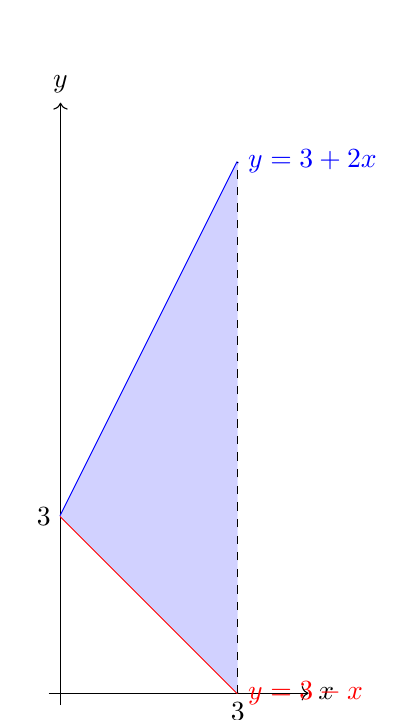
\begin{tikzpicture}[scale=0.75]
\draw[->] (-0.2,0) -- (4.2,0) node[right] {$x$};
\draw[->] (0,-0.2) -- (0,10) node[above] {$y$};
\draw[domain=0:3,smooth,thick,blue] plot (\x,{3+2*\x}) node[right] {$y=3+2x$};
\draw[domain=0:3,smooth,thick,red] plot (\x,{3-\x}) node[right] {$y=3-x$};
\fill[blue!18,domain=0:3,variable=\x]
(0,3) -- plot (\x,{3+2*\x}) -- (3,0) -- plot[domain=3:0] (\x,{3-\x}) -- cycle;
\draw[dashed] (3,0) -- (3,9);
\node[below] at (3,0) {$3$};
\node[left] at (0,3) {$3$};
\end{tikzpicture}
\end{center}

\finalans{\text{Area}=\frac{27}{2}\text{ square units}}

\question{5(b). Find the direction cosines of the line passing through the points $(1,2,3)$ and $(-1,1,0)$.}
\answer
The direction vector of the line is
\[
\vec d=(-1-1,\ 1-2,\ 0-3)=(-2,-1,-3).
\]
Its magnitude is
\[
|\vec d|=\sqrt{(-2)^2+(-1)^2+(-3)^2}=\sqrt{14}.
\]
Therefore, the direction cosines are
\[
l=\frac{-2}{\sqrt{14}},
\quad m=\frac{-1}{\sqrt{14}},
\quad n=\frac{-3}{\sqrt{14}}.
\]
If the opposite direction is chosen, all signs may be changed simultaneously.
\finalans{\left(-\frac2{\sqrt{14}},-\frac1{\sqrt{14}},-\frac3{\sqrt{14}}\right)}

\question{5(c). Find the maximum value of $2a+5b$ subject to
\[
-3a-2b\leq-6,
\quad -2a+b\leq2,
\quad 4a+6b\leq24,
\quad 2a-3b\leq3,
\quad a\geq0,
\quad b\geq0.
\]}
\answer
First rewrite the constraints:
\[
3a+2b\geq6,
\quad -2a+b\leq2,
\quad 2a+3b\leq12,
\quad 2a-3b\leq3,
\quad a,b\geq0.
\]
The corner points of the feasible region are obtained from intersections of boundary lines. The relevant vertices are
\[
\left(\frac25,\frac{12}{5}\right),
\quad
\left(\frac65,\frac{16}{5}\right),
\quad
\left(\frac{24}{13},\frac3{13}\right),
\quad
\left(\frac{15}{4},\frac32\right).
\]
Evaluate $Z=2a+5b$ at these vertices:
\[
\begin{array}{c|c}
(a,b)&Z=2a+5b\\\hline
\left(\frac25,\frac{12}{5}\right)&\frac{64}{5}\\
\left(\frac65,\frac{16}{5}\right)&\frac{92}{5}\\
\left(\frac{24}{13},\frac3{13}\right)&\frac{63}{13}\\
\left(\frac{15}{4},\frac32\right)&15
\end{array}
\]
The maximum is $\frac{92}{5}$ at $\left(\frac65,\frac{16}{5}\right)$.

\begin{center}
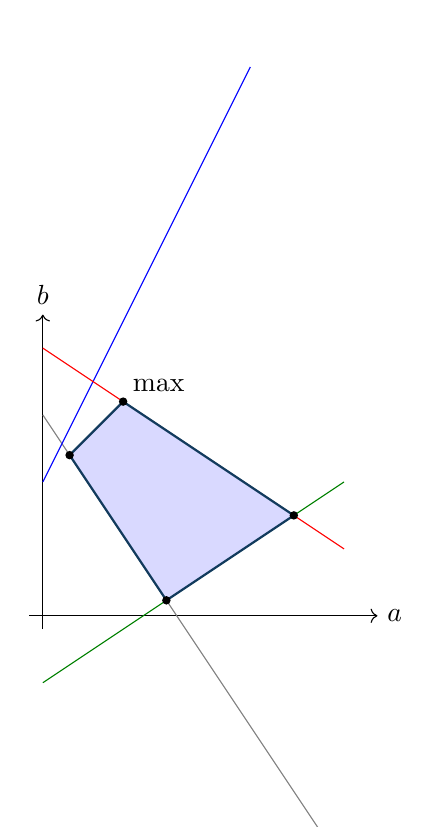
\begin{tikzpicture}[scale=0.85]
\draw[->] (-0.2,0)--(5,0) node[right] {$a$};
\draw[->] (0,-0.2)--(0,4.5) node[above] {$b$};
\draw[domain=0:4.2,smooth,gray] plot (\x,{(6-3*\x)/2});
\draw[domain=0:3.1,smooth,blue] plot (\x,{2+2*\x});
\draw[domain=0:4.5,smooth,red] plot (\x,{(12-2*\x)/3});
\draw[domain=0:4.5,smooth,green!50!black] plot (\x,{(2*\x-3)/3});
\filldraw[fill=blue!15,draw=headblue,thick]
(0.4,2.4)--(1.2,3.2)--(3.75,1.5)--(24/13,3/13)--cycle;
\foreach \x/\y/\lab in {0.4/2.4/{(2/5,12/5)},1.2/3.2/{(6/5,16/5)},3.75/1.5/{(15/4,3/2)},1.846/0.231/{(24/13,3/13)}}
{\fill (\x,\y) circle (1.8pt);}
\node[above right] at (1.2,3.2) {max};
\end{tikzpicture}
\end{center}

\finalans{Z_{\max}=\frac{92}{5}\text{ at }\left(a,b\right)=\left(\frac65,\frac{16}{5}\right)}

\question{5(d). Reduce the matrix
\[
A=\begin{bmatrix}5&3&8\\0&1&1\\1&-1&0\end{bmatrix}
\]
to normal form and hence find its rank.}
\answer
Use elementary row operations:
\[
A=\begin{bmatrix}5&3&8\\0&1&1\\1&-1&0\end{bmatrix}.
\]
Interchange $R_1$ and $R_3$:
\[
\begin{bmatrix}1&-1&0\\0&1&1\\5&3&8\end{bmatrix}.
\]
Apply $R_3\to R_3-5R_1$:
\[
\begin{bmatrix}1&-1&0\\0&1&1\\0&8&8\end{bmatrix}.
\]
Apply $R_3\to R_3-8R_2$:
\[
\begin{bmatrix}1&-1&0\\0&1&1\\0&0&0\end{bmatrix}.
\]
Apply $R_1\to R_1+R_2$:
\[
\begin{bmatrix}1&0&1\\0&1&1\\0&0&0\end{bmatrix}.
\]
By using elementary column operations, subtract column 1 from column 3, then subtract column 2 from column 3:
\[
\begin{bmatrix}1&0&0\\0&1&0\\0&0&0\end{bmatrix}.
\]
This is the normal form.
\finalans{\text{Normal form}=\begin{bmatrix}1&0&0\\0&1&0\\0&0&0\end{bmatrix},\quad \operatorname{rank}(A)=2}

\newpage
\section*{Theory and Formula Sheet Required for This Paper}

\begin{tcolorbox}[colback=softgreen,colframe=green!45!black,title={1. Determinants and matrices}]
\begin{itemize}[leftmargin=*]
\item If one row or column is a linear combination of others, the determinant is zero.
\item $A(\operatorname{adj}A)=|A|I$.
\item If $f(A)=0$, use it to reduce higher powers of $A$.
\item A matrix is in normal form $\operatorname{diag}(I_r,0)$, where $r$ is its rank.
\end{itemize}
\end{tcolorbox}

\begin{tcolorbox}[colback=softgreen,colframe=green!45!black,title={2. Algebra, sequences, induction}]
\begin{itemize}[leftmargin=*]
\item For $ax^2+bx+c=0$, sum of roots $=-b/a$, product of roots $=c/a$.
\item GP sum: $S_n=\dfrac{a(r^n-1)}{r-1}$, $r\ne1$.
\item Sum of cubes: $1^3+2^3+\cdots+n^3=\left[\dfrac{n(n+1)}{2}\right]^2$.
\item Mathematical induction: prove base case, assume $P(k)$, then prove $P(k+1)$.
\end{itemize}
\end{tcolorbox}

\begin{tcolorbox}[colback=softgreen,colframe=green!45!black,title={3. Complex numbers and cube roots of unity}]
\begin{itemize}[leftmargin=*]
\item Cube roots of unity are $1,\omega,\omega^2$ with $\omega^3=1$ and $1+\omega+\omega^2=0$.
\item De Moivre's theorem: $(\cos\theta+i\sin\theta)^n=\cos n\theta+i\sin n\theta$.
\item Write $a+ib=r(\cos\theta+i\sin\theta)$ before applying De Moivre's theorem.
\end{itemize}
\end{tcolorbox}

\begin{tcolorbox}[colback=softgreen,colframe=green!45!black,title={4. Calculus}]
\begin{itemize}[leftmargin=*]
\item For local maxima/minima, solve $f'(x)=0$ and use $f''(x)$: if $f''<0$, local maximum; if $f''>0$, local minimum.
\item Arc length: $L=\int_a^b\sqrt{1+(dy/dx)^2}\,dx$.
\item Area between curves: $A=\int_a^b(\text{upper curve}-\text{lower curve})\,dx$.
\item Rationalisation is useful for limits involving square roots.
\end{itemize}
\end{tcolorbox}

\begin{tcolorbox}[colback=softgreen,colframe=green!45!black,title={5. Three-dimensional geometry and vectors}]
\begin{itemize}[leftmargin=*]
\item Direction cosines of vector $(a,b,c)$ are $\left(\dfrac{a}{r},\dfrac{b}{r},\dfrac{c}{r}\right)$, where $r=\sqrt{a^2+b^2+c^2}$.
\item Three vectors are coplanar if their scalar triple product is zero.
\item Angle between lines with direction vectors $\vec a,\vec b$:
\[
\cos\theta=\frac{|\vec a\cdot\vec b|}{|\vec a||\vec b|}.
\]
\item Shortest distance between skew lines:
\[
d=\frac{|(\vec a_2-\vec a_1)\cdot(\vec b_1\times\vec b_2)|}{|\vec b_1\times\vec b_2|}.
\]
\end{itemize}
\end{tcolorbox}

\begin{tcolorbox}[colback=softgreen,colframe=green!45!black,title={6. Linear programming}]
\begin{itemize}[leftmargin=*]
\item Convert inequalities to boundary lines and find the feasible region.
\item The maximum or minimum of a linear objective function occurs at a corner point of the feasible region.
\item Evaluate the objective function at every feasible vertex and choose the best value.
\end{itemize}
\end{tcolorbox}

\end{document}
